\documentclass[11pt]{article}

% ---------- Packages ----------
\usepackage[margin=1in]{geometry}
\usepackage{amsmath, amssymb}
\usepackage{graphicx}
\usepackage{fancyhdr}
\usepackage{float}

% ---------- Paragraph Formatting ----------
\setlength{\parindent}{0pt}
\setlength{\parskip}{0.5em}

% ---------- Header ----------
\pagestyle{fancy}
\fancyhf{}
\lhead{ASEN 5335 Aerospace Environment}
\rhead{Justin Le}
\cfoot{\thepage}

% ---------- Document ----------
\begin{document}

% ---------- Title ----------
\begin{center}
    {\Large \textbf{Homework 2}}\\[0.5em]
    {\large ASEN 5335 Aerospace Environment}\\[0.5em]
    Justin Le\\ 
    \today
    \\[0.5em]
\end{center}

\vspace{1em}

\section*{Problem 1: Spaceballs}
\subsection*{(i.)}
\hspace*{2em}We are able to use the provided MSISatmosphere1000.m profile to calculate the
an approximate total mass of the atmosphere. The MSISatmosphere1000 function 
takes inputs of altitudes and outputs a structure, one of which is mass density which
corresponds to that altitude. Using MATLAB we are able to have a vector of altitudes that
range to 1000 km, the maximum model input of the MSISatmosphere1000 function. We can then 
obtain a vector of mass densities $\rho$. We use the following,
\[
\begin{gathered}
m = \rho V \\
m = \int{\rho dV} \\
\text{And for a sphere,} \\
m = \int{\rho*4\pi r^2 dr} \\
\therefore m = 4\pi\int{\rho r^2dr}
\end{gathered}
\]
\hspace*{2em}With $\rho$ being a vector and $r$ also being a vector of radius of this atmospheric
shell (altitude including radius of the Earth $R_E = 6371 \, \mathrm{km}$), we can integrate
within MATLAB to obtain a $\boxed{m=5.297*10^{18}\,\mathrm{kg}}$.
\subsection*{(ii.)}
\hspace*{2em}Assuming a volume of $V = 10*10^3*10*10^3*100*10^3 = 1*10^{13} \, \mathrm{m^3}$, a constant temperature $T = 300 \, \mathrm{K}$, molar mass $M = 0.029 \, \mathrm{kg/mol}$,
and universal gas constant $R = 8.314 \, \mathrm{J/(molK)}$. We can use the ideal gas law,
\[
\begin{gathered}
PV = \frac{m}{M}\\
\text{Rewrite to solve for pressure $P$,} \\
P = \frac{m}{MV}RT \\
\boxed{P = 4.556*10^{10} \, \mathrm{Pa}}
\end{gathered}
\]

\section*{Problem 2: Atmospheric Scale Height}
\hspace*{2em}To calculate the scale height $H$ of air mixture assuming $N_2/O_2$ mixture
at sea level, we use the equation.
\[
\begin{gathered}
H = \frac{kT}{mg}
\end{gathered}
\]
\hspace*{2em}Where we assume a constant $T = 300 \, \mathrm{K}$ from the problem, and $k = 1.38*10^{-23} \, \mathrm{J/K}$,
the Boltzmann constant, $g = 9.81 \, \mathrm{m/s^2}$, the gravitational constant. We then 
seek the molecular mass of $N_2/O_2$ mixture. This can be obtained from the table provided
in the HW. We find the atomic mass of the air mixture provided with the \% by volume
\[
\begin{gathered}
amu_{air} = 28.0134\left(.781\right)+31.9988\left(.209\right) = 28.566\, \mathrm{g/mol} \\
m_{air} = amu_{air}*\frac{1 \, \mathrm{kg}}{1000\, \mathrm{g} * 6.02*10^{23}\, \mathrm{g/mol}} \\
m_{air} = 4.745*10^{-26} \, \mathrm{kg}
\end{gathered}
\]

\hspace*{2em}This process of finding molecular weight and converting it can be repeated for
atomic Oxygen, helium, and hydrogen. 
\[
\begin{gathered}
amu_{oxygen} = (31.9988 \, \mathrm{g/mol}) / 2 = 15.9994 \, \mathrm{g/mol} \\
amu_{helium} = 4.0026  \, \mathrm{g/mol} \\
amu_{hydrogen} = 2.01594  \, \mathrm{g/mol}
\\
\\
m_{oxygen} = 2.6577*10^{-26} \, \mathrm{kg} \\
m_{helium} = 6.6488*10^{-27} \, \mathrm{kg} \\
m_{hydrogen} = 3.3487*10^{-27} \, \mathrm{kg}
\end{gathered}
\]

\hspace*{2em}The scale height equation can be used with each respective molecular mass of
the species in question.
\[
\begin{gathered}
\boxed{H_{air} = 8.8938*10^3 \, \mathrm{m}} \\
\boxed{H_{oxygen} = 1.588*10^4 \, \mathrm{m}} \\
\boxed{H_{helium} = 6.347*10^4 \, \mathrm{m}} \\
\boxed{H_{hydrogen} = 1.2602*10^5 \, \mathrm{m}}
\end{gathered}
\]


\begin{figure}[H]
    \centering
    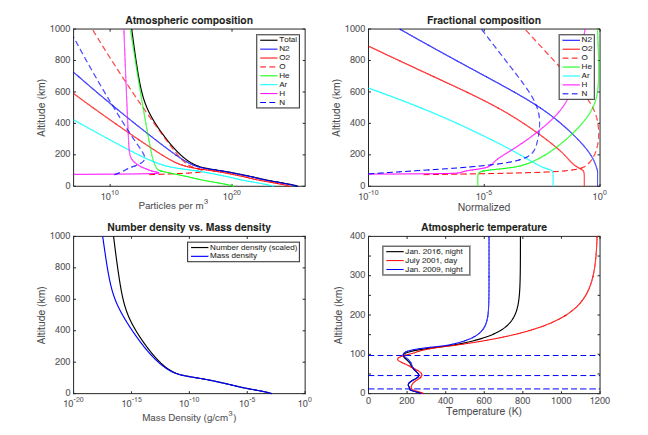
\includegraphics[width=0.8\textwidth]{atmospheric_profile.png}
    \caption{Atmospheric Profile}
    \label{fig:atmospheric_profile}
\end{figure}


By comparing these scale heights to those in the Figure 1 provided from the HW,
we observe that 

TODO: We seek to also calculate scale height from the MSIS profiles. From the MSIS
profiles there will be different temperatures instead of the fixed $T$ used earlier.
Using altitudes of 150,180,450,500,600,1000km.

\section*{Problem 3: Atmosphere Variation}
\subsection*{(i.)}
\begin{figure}[H]
    \centering
    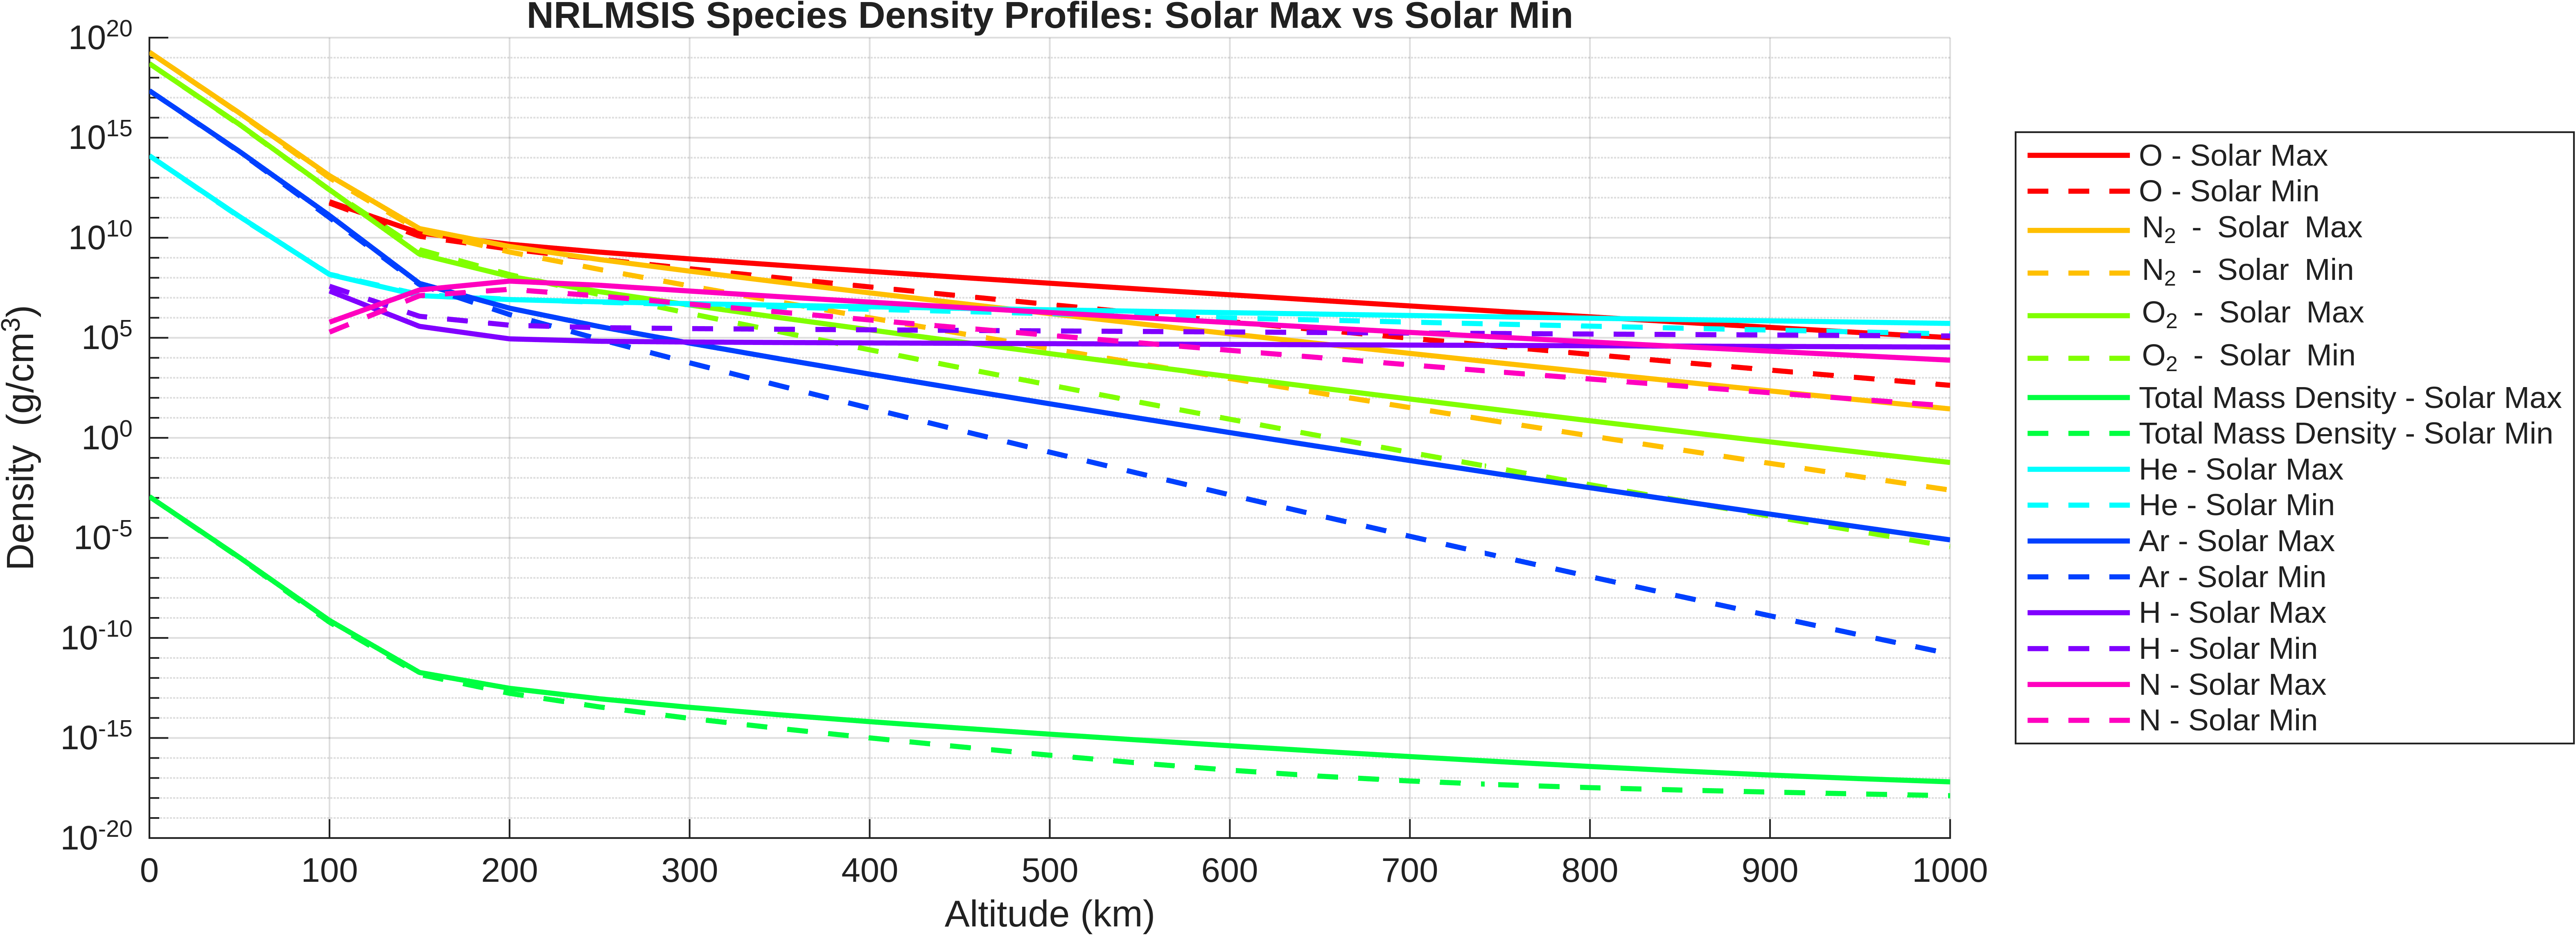
\includegraphics[width=0.8\textwidth]{NRLMSIS_Species_Density_Profiles.png}
    \caption{NRLMSIS Species Density Profiles Solar Max vs Solar Min}
    \label{fig:NRLMSIS_Species_Density_Profiles}
\end{figure}

\subsection*{(ii.)}
\hspace*{2em}At 600 km, there is variation between the solar maximum and solar minimum with the
density profiles of each species deviating. At solar maximums, the densities of each
species tends to be larger by multiple orders of magnitude than they would be a solar minimums.
This can even be soon overall with the Total Mass Density variation between solar maximums and
minimums. The implication of this for spacecraft operations is that there will be different atmospheric conditions
for spacecraft depending on if it is a solar maximum or minimum. For instance, drag will be
dependent on the density of the atmosphere, during solar maximums where density can increase
by multiple orders of magnitude, drag will also be considerably affected. This could especially
impact LEO orbits with their orbits being considerably influenced by drag. Their satellite operations
could therefore vary depending on if it is a solar maximum or minimum. 

\subsection*{(iii.)}
\hspace*{2em}The dominant atmospheric constituent would be O, atomic oxygen, for both solar
maximum and solar minimum. (TODO: Double check this...)
\section*{Problem 4: Oxygen Impact}
\subsection*{(i.)}
\hspace*{2em}To find the characteristic velocity of an oxygen atom O at $T = 1000 \, \mathrm{K}$ in the thermosphere,
we are able to use the Maxwell Boltzmann Characteristic RMS Velocity equation.
\[
\begin{gathered}
v_{rms} = \sqrt{ \frac{3k_B T}{m} }
\end{gathered}
\]
\hspace*{2em}$k_B = 1.38*10^{-23} \, mathrm{m^2 kg / s^2 K}$ as the Boltzmann constant, and 
we are able to find $m = 2.657*10^{-26} \, \mathrm{kg}$ for an oxygen atom. We can plug this
into the equation to simply find,
\[
\begin{gathered}
\boxed{v = 1248.26 \, \mathrm{m/s}}    
\end{gathered}
\]

\subsection*{(ii.)}
\hspace*{2em}We then calculate the velocity that a 
spacecraft in LEO at 600 km would have,
\[
\begin{gathered}
v_{orbit} = \sqrt{\frac{GM_{Earth}}{r}} \\
G = 6.67*10^{-11} \, \mathrm{Nm^2/kg^2} \\
M_{Earth} = 5.972*10^{24} \, \mathrm{kg} \\
r = 600*10^3 \, \mathrm{m} + 6371*10^3 \, \mathrm{m} = 6671*10^3 \, \mathrm{m} \\
\therefore v_{orbit} = 7559 \, \mathrm{m/s}
\end{gathered}
\]

The energy imparted onto the spacecraft by an oxygen atom would be using the mass
of the oxygen atom and the velocity of the spacecraft,
\[
\begin{gathered}
KE = \frac{1}{2} m_{oxygen} v_{orbit}^2 \\
KE = 7.591*10^{-19} J \\
\text{Where $1\, \mathrm{J}$ = $6.242*10^{18} \, \mathrm{eV}$} \\
\boxed{\therefore KE = 4.738 \, \mathrm{eV}}
\end{gathered}
\]

\subsection*{(iii.)}
TODO: TODO

\section*{Problem 5: Orbit Decay}
\subsection*{(i.)}
\[
\begin{gathered}
\text{We use the following relations:} \\
F_{drag} = \frac{1}{2} \rho V^2 C_D A, \qquad
V = \sqrt{\frac{G M_E}{a}}, \qquad
P^2 G M_E = 4 \pi^2 a^3
\end{gathered}
\]

\[
\begin{gathered}
\textbf{Step 1:} \text{ Drag equation} \\
m \frac{dV}{dt} = \frac{1}{2} \rho V^2 C_D A \\
\frac{dV}{dt} = \frac{\rho V^2 C_D A}{2m}
\end{gathered}
\]

\[
\begin{gathered}
\textbf{Step 2:} \text{ Relate } da/dt \text{ to } dV/dt \text{ with the velocity equation} \\
V^2 a = G M_E \\
\left(\frac{d}{dt}\right)\Big(V^2 a\Big) = \left(\frac{d}{dt}\right)\Big(G M_E\Big) \\
2Va\,\frac{dV}{dt} + V^2 \frac{da}{dt} = 0 \\
\frac{da}{dt} = -\frac{2a}{V}\frac{dV}{dt} \\
\text{Substituting Step 1,} \\
\frac{da}{dt} = -\frac{2a}{V}\left(\frac{\rho V^2 C_D A}{2m}\right) \\
\frac{da}{dt} = -\frac{a \rho V C_D A}{m}
\end{gathered}
\]

\[
\begin{gathered}
\textbf{Step 3:} \text{ Relate } da/dt \text{ to } dP/dt \text{ with Kepler's third law} \\
P^2 G M_E = 4 \pi^2 a^3 \\
\left(\frac{d}{dt}\right)\Big(P^2 G M_E\Big) = \left(\frac{d}{dt}\right)\Big(4 \pi^2 a^3\Big) \\
2P\,G M_E\,\frac{dP}{dt} = 12\pi^2 a^2 \frac{da}{dt} \\
\frac{da}{dt} = \frac{P\,G M_E}{6 \pi^2 a^2}\,\frac{dP}{dt}
\end{gathered}
\]

\[
\begin{gathered}
\textbf{Step 4:} \text{ Setting the two expressions for $da/dt$ equal,} \\
-\frac{a \rho V C_D A}{m} = \frac{P\,G M_E}{6 \pi^2 a^2}\,\frac{dP}{dt} \\
\frac{dP}{dt} = -\frac{6 \pi^2 a^3 \rho V C_D A}{m\,P\,G M_E} \\
\text{Using } GM_E = V^2 a \text{ to eliminate } GM_E, \\
\frac{dP}{dt} = -\frac{6 \pi^2 a^3 \rho V C_D A}{m\,P\,V^2 a} \\
\frac{dP}{dt} = -\frac{6 \pi^2 a^2 \rho C_D A}{m\,P\,V} \\
\text{For a circular orbit, } 2\pi a = PV, \\
\frac{dP}{dt} = -\frac{6 \pi^2 a^2}{m\,(2\pi a)}\,\rho C_D A \\
\frac{dP}{dt} = -\frac{3 \pi a \rho C_D A}{m}
\end{gathered}
\]
\[
\boxed{\frac{dP}{dt} = -3 \pi a \rho \frac{C_D A}{m}}
\]
\subsection*{(ii.)}
\hspace*{2em} See section at end of assignment for full MATLAB Code. 
\begin{figure}[H]
    \centering
    
\includegraphics[width=0.6\textwidth]{HW2Problem5_OrbitDecay_400km_x.png}
    \caption{Orbital Decay for 400 km in +x}
    \label{fig:HW2Problem5_OrbitDecay_400km_x}
\end{figure}
\subsection*{(iii.)}
\begin{figure}[H]
    \centering
    
\includegraphics[width=0.6\textwidth]{HW2Problem5_OrbitDecay_500km_x.png}
    \caption{Orbital Decay for 500 km in +x}
    \label{fig:HW2Problem5_OrbitDecay_500km_x}
\end{figure}
\subsection*{(iv.)}
\begin{figure}[H]
    \centering
    
\includegraphics[width=0.6\textwidth]{HW2Problem5_OrbitDecay_400km_z.png}
    \caption{Orbital Decay for 400 km in +z}
    \label{fig:HW2Problem5_OrbitDecay_400km_z}
\end{figure}

\section*{Problem 6: Atmosphere Uncertainty and Neutral Winds}
\subsection*{(i.)}
\begin{figure}[H]
    \centering
    
\includegraphics[width=0.6\textwidth]{HW2Problem6_OrbitDecay_400km_x_uncertainty.png}
    \caption{Orbital Decay for 400 km in +z with 10\% Uncertainty}
    \label{fig:HW2Problem5_OrbitDecay_400km_uncertain_z}
\end{figure}

\hspace*{2em}We are able to observe a difference in deorbit time of between 
33 and 34 days based on the upper and lower bounds of density uncertainty.
\subsection*{(ii.)}
\hspace*{2em}Given a 90 minute orbit around Earth at some LEO altitude where this
cubesat is operating, the implications for where this spacecraft re entry point in the
atmosphere is that there is massive uncertainty in where it will re enter the atmosphere
over it's entire ballistic deorbiting process. This location would greatly vary due to 
this uncertainty.

\section*{Problem 7: Air Breathing Thruster}

\section*{Problem 8: Missions}

\newpage
\section*{MATLAB Code}

\begin{verbatim}
%% ASEN 5335 Aerospace Environment
%% Justin Le
%% HW2 Problem 5

clc;clear; close all

% Constants
G = 6.67e-11;
M_E = 5.972e24;
R_E_m = 6371e3;
C_D = 2.2;
m_sat_kg = 4; % From earlier in notes
A_x_m2 = 0.09;
A_z_m2 = 0.01;
stop_alt_km = 120;

% Part ii, 400 km altitude in +x direction
[t2_days, alt2_km] = simulateDecay(400, A_x_m2, stop_alt_km, G, M_E, R_E_m, C_D, m_sat_kg);
% Part iii, 500 km in +x direction
[t3_days, alt3_km] = simulateDecay(500, A_x_m2, stop_alt_km, G, M_E, R_E_m, C_D, m_sat_kg);
% Part iv, 400 km altitude in +z direction
[t4_days, alt4_km] = simulateDecay(400, A_z_m2, stop_alt_km, G, M_E, R_E_m, C_D, m_sat_kg);

figure
plot(t2_days, alt2_km)
grid on
xlabel('Time (days)')
ylabel('Altitude (km)')
title('Orbital Decay: 400 km Start, Ram in +X')
set(gcf, 'Units', 'inches', 'Position', [0 0 6 4])
exportgraphics(gcf, 'HW2Problem5_OrbitDecay_400km_x.png', 'Resolution', 600);

figure
plot(t3_days, alt3_km)
grid on
xlabel('Time (days)')
ylabel('Altitude (km)')
title('Orbital Decay: 500 km Start, Ram in +X')
set(gcf, 'Units', 'inches', 'Position', [0 0 6 4])
exportgraphics(gcf, 'HW2Problem5_OrbitDecay_500km_x.png', 'Resolution', 600);

figure
plot(t4_days, alt4_km)
grid on
xlabel('Time (days)')
ylabel('Altitude (km)')
title('Orbital Decay: 400 km Start, Ram in +Z')
set(gcf, 'Units', 'inches', 'Position', [0 0 6 4])
exportgraphics(gcf, 'HW2Problem5_OrbitDecay_400km_z.png', 'Resolution', 600);

function [t_days, alt_km] = simulateDecay(alt0_km, A_m2, stop_alt_km, G, M_E, R_E_m, C_D, m_sat)
% Calculate orbital elements at this time point
a = R_E_m + alt0_km*1000;
P = 2*pi*sqrt(a^3/(G*M_E));

% Conditions to iterate
t = 0;
altitude_index = 1;
t_hist(altitude_index) = 0;
alt_hist(altitude_index) = alt0_km;

% At start, alt = alt0.
alt_current_km = alt0_km;
% Loop until sat deorbits
while alt_current_km > stop_alt_km
    % Find density at that altitude
    MSIS = MSISatmosphere1000(alt_current_km);
    rho = MSIS.mass*1000;
    
    % Equation 10 and find change in Period
    dPdt = -3*pi*a*rho*C_D*A_m2/m_sat;
    
    dt = 600;

    P = P + dPdt*dt;
    t = t + dt;

    a = (G*M_E*P^2/(4*pi^2))^(1/3);
    alt_current_km = (a - R_E_m)/1000

    altitude_index = altitude_index + 1;
    t_hist(altitude_index) = t/86400; % Convert to days
    alt_hist(altitude_index) = alt_current_km;
end

t_days = t_hist;
alt_km = alt_hist;

end
\end{verbatim}

\end{document}
